\documentclass{article}
\usepackage{tikz}
\usepackage{xspace}
\newcommand{\hackenbush}{\textup{\textsc{Hackenbush}}\xspace}

\begin{document}

\begin{figure}[h]
\centering
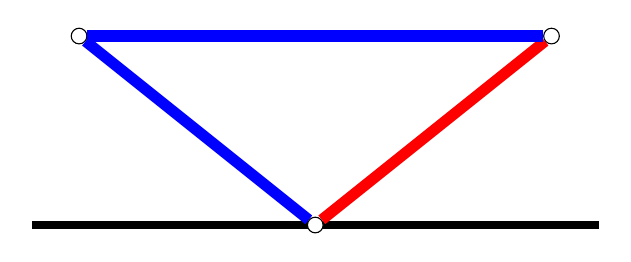
\begin{tikzpicture}[scale=1.2]
    % Ground line
    \draw[line width=3pt] (-3,0) -- (3,0);
    
    % Vertices
    \node[circle, draw, fill=white, inner sep=2pt] (bottom) at (0,0) {};
    \node[circle, draw, fill=white, inner sep=2pt] (left) at (-2.5,2) {};
    \node[circle, draw, fill=white, inner sep=2pt] (right) at (2.5,2) {};
    
    % Edges
    \draw[line width=4pt, blue] (bottom) -- (left);
    \draw[line width=4pt, red] (bottom) -- (right);
    \draw[line width=4pt, blue] (left) -- (right);
\end{tikzpicture}
\caption{A game of \hackenbush, with literal form $\{ 1-1,-\frac{1}{2} \mathrel\vert \{ 0,1 \mathrel\vert \} \}$, that is not a conflict placement game. This game is not a conflict placement game because the top edge cannot be cut if both bottom edges are cut, but the top edge can be cut if at most one of the bottom edges is cut.}
\end{figure}

\end{document}